

\begin{figure}[ht]
	\centerline{
\includegraphics[width=0.80\textwidth]{Gambar/dapi2.jpg}}
	\caption{Exceptions reguler}
	\label{Exceptions reguler}
\end{figure}

\section {Pengertian }
\subsection {Exceptions reguler}
Exceptions reguler adalah urutan khusus karakter yang membantu Anda mencocokkan atau menemukan string atau rangkaian senar lainnya, menggunakan sintaks khusus yang dipegang dalam sebuah pola. Ekspresi reguler banyak digunakan di dunia UNIX. Modul ini memberikan dukungan penuh untuk ekspresi reguler seperti Perl dengan Python. Modul re meningkatkan pengecualian re.error jika terjadi kesalahan saat mengkompilasi atau menggunakan ekspresi reguler.Kami akan membahas dua fungsi penting, yang akan digunakan untuk menangani ekspresi reguler. Tapi ada hal kecil dulu: Ada berbagai karakter, yang tentunya memiliki arti khusus bila digunakan dalam ekspresi reguler. Untuk menghindari kebingungan saat berhadapan dengan ekspresi reguler, kita akan menggunakan Raw Strings sebagai r'expression '. \par
\vspace{14pt}
\noindent


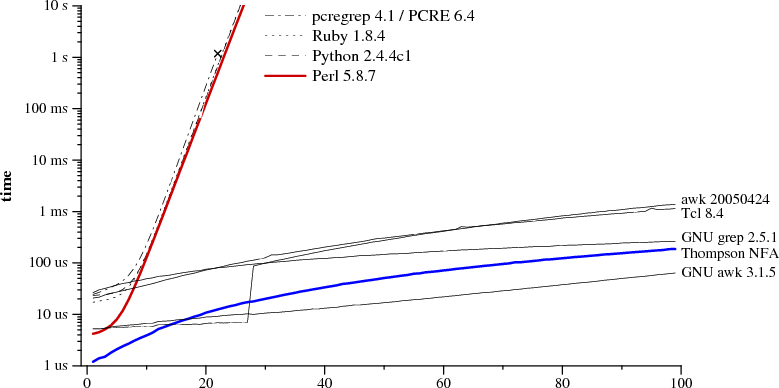
\includegraphics[width=10cm,height=7cm]{Gambar/dapi1.jpg}
\begin{equation}python regular expression\end{equation}

 \section{Berikut adalah sintaks untuk fungsi ini }
 
 \begin{itemize}
\item Fungsi Pertandingan \par
\noindent 
Fungsi ini mencoba mencocokkan pola RE dengan string dengan flag pilihan. \par
\vspace{12pt}
\noindent 

\noindent 
  \par
\noindent 

\item Parameter 
\noindent 
pattern \hspace*{0.5in}  \par
\noindent 
Ini adalah ekspresi reguler yang harus disesuaikan. \par
\vspace{12pt}
\noindent 
\item string 
\noindent 
Ini adalah string, yang akan dicari agar sesuai dengan pola pada awal string. \par
\vspace{12pt}
\noindent 
\item flags 

Anda dapat menentukan flag yang berbeda menggunakan bitwise OR ( $  \vert  $). Ini adalah pengubah, yang tercantum dalam tabel di bawah ini. \par
\vspace{12pt}
\vspace{12pt}

\item Fungsi re.match  
 
mengembalikan objek yang cocok pada kesuksesan, None on failure. Kami mengelompokkan (num) atau kelompok () fungsi objek pencocokan untuk mendapatkan ekspresi yang sesuai. \par
\noindent 


\item Match Object Methods 
 
group(num=0) \hspace*{0.5in} Metode ini mengembalikan seluruh kecocokan (atau jumlah subkelompok tertentu) \par
\vspace{12pt}
groups() \hspace*{0.5in}  \par
\noindent 
Metode ini mengembalikan semua subkelompok yang cocok dalam tupel (kosong jika tidak ada) \par
\vspace{12pt}
\vspace{12pt}
\noindent

\end{itemize} 

\begin{verbatim}
 $  \#  $! / Usr / bin / python \par
\noindent 
Impor kembali \par
\vspace{12pt}
\noindent 
Line = "Kucing lebih pintar dari pada anjing" \par
\vspace{12pt}
\noindent 
MatchObj = re.match (r '(. *) Adalah (. *?). *', Line, re.M  $  \vert  $ re.I) \par
\vspace{12pt}
\noindent 
jika cocokObj: \par
\noindent 
~~ cetak "matchObj.group ():", matchObj.group () \par
\noindent 
~~ cetak "matchObj.group (1):", matchObj.group (1) \par
\noindent 
~~ Cetak "matchObj.group (2):", matchObj.group (2) \par
\noindent 
lain: \par
\noindent 
~~ cetak "Tidak ada pertandingan !!" \par
\vspace{12pt}
\noindent 
Bila kode diatas dieksekusi, maka menghasilkan hasil sebagai berikut - \par
\vspace{12pt}
\noindent 
MatchObj.group (): Kucing lebih pintar dari pada anjing \par
\noindent 
MatchObj.group (1): Kucing \par
\noindent 
MatchObj.group (2): lebih pintar \par

\end{verbatim}

\vspace{12pt}
\section{Fungsi Pencarian} \par
\vspace{12pt}
Fungsi ini mencari kejadian pertama dari pola RE dalam string dengan flag pilihan. \par
\vspace{12pt}

\subsection{Pengertian}
Berikut adalah sintaks untuk fungsi ini: \par
\vspace{12pt}
Re.search (pola, string, flag = 0) \par
\vspace{12pt}
\noindent 
Berikut adalah deskripsi parameternya: \par
Parameter pattern Ini adalah ekspresi reguler yang harus disesuaikan. String Ini adalah string, yang akan dicari agar sesuai dengan pola di manapun dalam string. Flags Anda dapat menentukan flag yang berbeda menggunakan bitwise OR ( $  \vert  $). Ini adalah pengubah, yang tercantum dalam tabel di bawah ini.Fungsi re.search mengembalikan objek yang cocok pada kesuksesan, tidak ada yang gagal. Kami menggunakan fungsi kelompok (num) atau kelompok () dari objek pertandingan untuk mendapatkan ekspresi yang sesuai.Match Object Methods Descriptiongroup(num=0) Metode ini mengembalikan seluruh kecocokan (atau jumlah subkelompok tertentu)groups()Metode ini mengembalikan semua subkelompok yang cocok dalam tupel (kosong jika tidak ada) \par
\vspace{12pt}
\vspace{12pt}
\noindent 

\begin{verbatim}
 $  \#  $!/usr/bin/python \par
\noindent 
import re \par
\vspace{12pt}
\noindent 
line = "Cats are smarter than dogs"; \par
\vspace{12pt}
\noindent 
searchObj = re.search( r'(.*) are (.*?) .*', line, re.M $  \vert  $re.I) \par
\vspace{12pt}
\noindent 
if searchObj: \par
\noindent 
~~ print "searchObj.group() : ", searchObj.group() \par
\noindent 
~~ print "searchObj.group(1) : ", searchObj.group(1) \par
\noindent 
~~ print "searchObj.group(2) : ", searchObj.group(2) \par
\noindent 
else: \par
\noindent 
~~ print "Nothing found!!" \par
\vspace{12pt}
\noindent 
searchObj.group()~:  Cats are smarter than dogs \par
\noindent 
searchObj.group(1)~:  Cats \par
\noindent 
searchObj.group(2)~:  smarter \par
\noindent 
Pencocokan Versus Searching \par
\vspace{12pt}

\end{verbatim}



Python menawarkan dua operasi primitif yang berbeda berdasarkan ekspresi reguler: cek kecocokan untuk kecocokan hanya di awal string, sementara pencarian memeriksa kecocokan di manapun dalam string (inilah yang Perl lakukan secara default). \par
Contoh \par
\noindent 
 $  \#  $!/usr/bin/python \par
\noindent 
import re \par
\vspace{12pt}
\noindent 
line = "Cats are smarter than dogs"; \par
\vspace{12pt}
\noindent 
matchObj = re.match( r'dogs', line, re.M $  \vert  $re.I) \par
\noindent 
if matchObj: \par
\noindent 
~~ print "match --> matchObj.group() : ", matchObj.group() \par
\noindent 
else: \par
\noindent 
~~ print "No match!!" \par
\vspace{12pt}
\noindent 
searchObj = re.search( r'dogs', line, re.M $  \vert  $re.I) \par
\noindent 
if searchObj: \par
\noindent 
~~ print "search --> searchObj.group() : ", searchObj.group() \par
\noindent 
else: \par
\noindent 
~~ print "Nothing found!!" \par
\vspace{12pt}
\noindent 
No match!! \par
\noindent 
search~--> matchObj.group() :  dogs \par
\vspace{12pt}
\noindent 
Cari dan Ganti \par
\vspace{12pt}
\noindent 
Salah satu metode re yang paling penting yang menggunakan ekspresi reguler adalah sub. \par
\noindent 
Sintaksis \par
\vspace{12pt}
Re.sub (pola, repl, string, max = 0) \par
\vspace{12pt}
\noindent 
Metode ini menggantikan semua kemunculan pola RE dalam string dengan repl, mengganti semua kejadian kecuali jika max diberikan. Metode ini mengembalikan string yang dimodifikasi. \par
Contoh \par
\noindent 
 $  \#  $!/usr/bin/python \par
\noindent 
import re \par
\vspace{12pt}
\noindent 
phone = "2004-959-559  $  \#  $ This is Phone Number" \par
\vspace{12pt}
\noindent 
 $  \#  $ Delete Python-style comments \par
\noindent 
num = re.sub(r' $  \#  $.* $  \$  $', "", phone) \par
\noindent 
print "Phone Num : ", num \par
\vspace{12pt}
\noindent 
 $  \#  $ Remove anything other than digits \par
\noindent 
num~=~re.sub(r' $  \textbackslash  $D',~"", phone)     \par
\noindent 
print "Phone Num : ", num \par
\vspace{12pt}
\noindent 
Phone~Num :  2004-959-559 \par
\noindent 
Phone~Num :  2004959559 \par
\vspace{12pt}
\noindent 
Regular Expression Modifiers: Option Flags \par
Ekspresi reguler literal mungkin termasuk pengubah opsional untuk mengendalikan berbagai aspek pencocokan. Pengubah ditentukan sebagai bendera pilihan. Anda dapat memberikan beberapa pengubah menggunakan OR eksklusif ( $  \vert  $), seperti yang ditunjukkan sebelumnya dan dapat ditunjukkan oleh salah satu dari ini – Modifier Description  \par
\noindent 
re.I \hspace*{0.5in}  \par
\noindent 
Lakukan pencocokan case-insensitive. \par
\vspace{12pt}
\noindent 
re.L \hspace*{0.5in}  \par
\noindent 
Menafsirkan kata-kata sesuai dengan lokal saat ini. Interpretasi ini mempengaruhi kelompok abjad ( $  \textbackslash  $ w dan  $  \textbackslash  $ W), serta perilaku batas kata ( $  \textbackslash  $ b dan  $  \textbackslash  $ B). \par
\vspace{12pt}
\noindent 
re.M \hspace*{0.5in}  \par
\noindent 
Membuat  $  \$  $ cocok dengan akhir baris (bukan hanya akhir string) dan membuat  $  \string^  $ cocok dengan awal baris apapun (bukan hanya permulaan string). \par
\vspace{12pt}
\noindent 
re.S \hspace*{0.5in}  \par
\noindent 
Membuat sebuah periode (dot) cocok dengan karakter apapun, termasuk newline. \par
\noindent 
re.U \hspace*{0.5in}  \par
\noindent 
Menginterpretasikan huruf sesuai dengan karakter Unicode. Flag ini mempengaruhi perilaku  $  \textbackslash  $ w,  $  \textbackslash  $ W,  $  \textbackslash  $ b,  $  \textbackslash  $ B. \par
\vspace{12pt}
\noindent 
re.X \hspace*{0.5in}  \par
\noindent 
Memungkinkan sintaks ekspresi reguler "manis". Ini mengabaikan spasi (kecuali di dalam himpunan [] atau saat diloloskan oleh garis miring terbalik) dan memperlakukan unescaped  $  \#  $ sebagai tanda komentar. \par
\vspace{12pt}
\noindent 
\textbf{Pola Ekspresi Reguler} \par
\vspace{12pt}
\noindent 
Kecuali karakter kontrol, (+?.  $  \string^  $  $  \string^  $  $  \$  $ () []  $  \{  $ $  \}  $  $  \vert  $  $  \textbackslash  $), Semua karakter cocok dengan karakter mereka sendiri. Anda bisa lolos dari karakter kontrol sebelum mendahului dengan garis miring terbalik. \par
\noindent 
Berikut daftar tabel sintaks ekspresi reguler yang tersedia dengan Python - \par
\noindent 
 $  \#  $!/usr/bin/python \par
\noindent 
import re \par
\vspace{12pt}
\noindent 
phone = "2004-959-559  $  \#  $ This is Phone Number" \par
\vspace{12pt}
\noindent 
 $  \#  $ Delete Python-style comments \par
\noindent 
num = re.sub(r' $  \#  $.* $  \$  $', "", phone) \par
\noindent 
print "Phone Num : ", num \par
\vspace{12pt}
\noindent 
 $  \#  $ Remove anything other than digits \par
\noindent 
num~=~re.sub(r' $  \textbackslash  $D',~"", phone)     \par
\noindent 
print "Phone Num : ", num \par
\vspace{12pt}
\noindent 
Phone~Num :  2004-959-559 \par
\noindent 
Phone~Num :  2004959559 \par
\vspace{12pt}
\noindent 
<Directory "/var/www/cgi-bin"> \par
\noindent 
~~ AllowOverride None \par
\noindent 
~~ Options ExecCGI \par
\noindent 
~~ Order allow,deny \par
\noindent 
~~ Allow from all \par
\noindent 
</Directory> \par
\vspace{12pt}
\noindent 
<Directory "/var/www/cgi-bin"> \par
\noindent 
Options All \par
\noindent 
</Directory> \par
\vspace{12pt}
\noindent 
!/usr/bin/python \par
\vspace{12pt}
\noindent 
print "Content-type:text/html $  \textbackslash  $r $  \textbackslash  $n $  \textbackslash  $r $  \textbackslash  $n" \par
\noindent 
print '<html>' \par
\noindent 
print '<head>' \par
\noindent 
print '<title>Hello Word - First CGI Program</title>' \par
\noindent 
print '</head>' \par
\noindent 
print '<body>' \par
\noindent 
print '<h2>Hello Word! This is my first CGI program</h2>' \par
\noindent 
print '</body>' \par
\noindent 
print '</html>' \par
\vspace{12pt}
\vspace{12pt}
\noindent 
Halo kata! Ini adalah program CGI pertamaku \par
\vspace{12pt}
Script hello.py ini adalah skrip Python yang sederhana, yang menuliskan hasilnya pada file STDOUT, yaitu layar. Ada satu fitur penting dan tambahan yang tersedia yang merupakan baris pertama yang akan dicetak Content-type: text / html  $  \textbackslash  $ r  $  \textbackslash  $ n  $  \textbackslash  $ r  $  \textbackslash  $ n. Baris ini dikirim kembali ke browser dan ini menentukan jenis konten yang akan ditampilkan di layar browser. Sekarang Anda pasti sudah mengerti konsep dasar CGI dan Anda bisa menulis banyak program CGI yang rumit dengan menggunakan Python. Script ini bisa berinteraksi dengan sistem eksternal lainnya juga untuk bertukar informasi seperti RDBMS. \par
\vspace{12pt}
\vspace{12pt}
\vspace{12pt}
\vspace{12pt}
\noindent 
Header HTTP \par
\vspace{12pt}
\noindent 
Baris Content-type: text / html  $  \textbackslash  $ r  $  \textbackslash  $ n  $  \textbackslash  $ r  $  \textbackslash  $ n adalah bagian dari header HTTP yang dikirim ke browser untuk memahami isinya. Semua header HTTP akan berada dalam bentuk berikut - \par
\noindent 
 $  \#  $!/usr/bin/python \par
\vspace{12pt}
\noindent 
 $  \#  $ Import modules for CGI handling  \par
\noindent 
import cgi, cgitb  \par
\vspace{12pt}
\noindent 
 $  \#  $ Create instance of FieldStorage  \par
\noindent 
form = cgi.FieldStorage()  \par
\vspace{12pt}
\noindent 
 $  \#  $ Get data from fields \par
\noindent 
first $  \_  $name = form.getvalue('first $  \_  $name') \par
\noindent 
last $  \_  $name~ = form.getvalue('last $  \_  $name') \par
\vspace{12pt}
\noindent 
print "Content-type:text/html $  \textbackslash  $r $  \textbackslash  $n $  \textbackslash  $r $  \textbackslash  $n" \par
\noindent 
print "<html>" \par
\noindent 
print "<head>" \par
\noindent 
print "<title>Hello - Second CGI Program</title>" \par
\noindent 
print "</head>" \par
\noindent 
print "<body>" \par
\noindent 
print "<h2>Hello  $  \%  $s  $  \%  $s</h2>"  $  \%  $ (first $  \_  $name, last $  \_  $name) \par
\noindent 
print "</body>" \par
\noindent 
print "</html>" \par
\vspace{12pt}
\noindent 
<form action="/cgi-bin/hello $  \_  $get.py" method="get"> \par
\noindent 
First~Name: <input type="text" name="first $  \_  $name">  <br /> \par
\vspace{12pt}
\noindent 
Last Name: <input type="text" name="last $  \_  $name" /> \par
\noindent 
<input type="submit" value="Submit" /> \par
\noindent 
</form> \par
\vspace{12pt}
\noindent 
 $  \#  $!/usr/bin/python \par
\vspace{12pt}
\noindent 
 $  \#  $ Import modules for CGI handling  \par
\noindent 
import cgi, cgitb  \par
\vspace{12pt}
\noindent 
 $  \#  $ Create instance of FieldStorage  \par
\noindent 
form = cgi.FieldStorage()  \par
\vspace{12pt}
\noindent 
 $  \#  $ Get data from fields \par
\noindent 
first $  \_  $name = form.getvalue('first $  \_  $name') \par
\noindent 
last $  \_  $name~ = form.getvalue('last $  \_  $name') \par
\vspace{12pt}
\noindent 
print "Content-type:text/html $  \textbackslash  $r $  \textbackslash  $n $  \textbackslash  $r $  \textbackslash  $n" \par
\noindent 
print "<html>" \par
\noindent 
print "<head>" \par
\noindent 
print "<title>Hello - Second CGI Program</title>" \par
\noindent 
print "</head>" \par
\noindent 
print "<body>" \par
\noindent 
print "<h2>Hello  $  \%  $s  $  \%  $s</h2>"  $  \%  $ (first $  \_  $name, last $  \_  $name) \par
\noindent 
print "</body>" \par
\noindent 
print "</html>" \par
\vspace{12pt}
\noindent 
<form action="/cgi-bin/hello $  \_  $get.py" method="post"> \par
\noindent 
First Name: <input type="text" name="first $  \_  $name"><br /> \par
\noindent 
Last Name: <input type="text" name="last $  \_  $name" /> \par
\vspace{12pt}
\noindent 
<input type="submit" value="Submit" /> \par
\noindent 
</form> \par
\vspace{12pt}
Mari kita ambil lagi contoh yang sama seperti di atas yang melewati dua nilai menggunakan HTML FORMULIR dan tombol kirim. Kami menggunakan skrip CGI yang sama hello $  \_  $get.py untuk menangani masukan ini. \par
\noindent 
Melewati Data Kotak Centang ke Program CGI \par
\vspace{12pt}
\noindent 
Kotak centang digunakan bila lebih dari satu pilihan diperlukan untuk dipilih. \par
\vspace{12pt}
\noindent 
Berikut adalah contoh kode HTML untuk form dengan dua kotak centang - \par
\vspace{12pt}
\noindent 
Melewati Data Tombol Radio ke Program CGI \par
\vspace{12pt}
\noindent 
Tombol Radio digunakan bila hanya satu pilihan yang harus dipilih. \par
\vspace{12pt}
\noindent 
Berikut adalah contoh kode HTML untuk form dengan dua tombol radio  \par
\vspace{12pt}
\vspace{12pt}
\noindent 
 $  \#  $!/usr/bin/python \par
\vspace{12pt}
\noindent 
 $  \#  $ Import modules for CGI handling  \par
\noindent 
import cgi, cgitb  \par
\vspace{12pt}
\noindent 
 $  \#  $ Create instance of FieldStorage  \par
\noindent 
form = cgi.FieldStorage()  \par
\vspace{12pt}
\noindent 
 $  \#  $ Get data from fields \par
\noindent 
if form.getvalue('subject'): \par
\noindent 
~~ subject = form.getvalue('subject') \par
\noindent 
else: \par
\noindent 
~~ subject = "Not set" \par
\vspace{12pt}
\noindent 
print "Content-type:text/html $  \textbackslash  $r $  \textbackslash  $n $  \textbackslash  $r $  \textbackslash  $n" \par
\noindent 
print "<html>" \par
\noindent 
print "<head>" \par
\noindent 
print "<title>Radio - Fourth CGI Program</title>" \par
\noindent 
print "</head>" \par
\noindent 
print "<body>" \par
\noindent 
print "<h2> Selected Subject is  $  \%  $s</h2>"  $  \%  $ subject \par
\noindent 
print "</body>" \par
\noindent 
print "</html>" \par
\vspace{12pt}
\noindent 
<form action="/cgi-bin/textarea.py" method="post" target=" $  \_  $blank"> \par
\noindent 
<textarea name="textcontent" cols="40" rows="4"> \par
\noindent 
Type your text here... \par
\noindent 
</textarea> \par
\noindent 
<input type="submit" value="Submit" /> \par
\noindent 
</form> \par
\vspace{12pt}
\noindent 
 $  \#  $!/usr/bin/python \par
\vspace{12pt}
\noindent 
 $  \#  $ Import modules for CGI handling  \par
\noindent 
import cgi, cgitb  \par
\vspace{12pt}
\noindent 
 $  \#  $ Create instance of FieldStorage  \par
\noindent 
form = cgi.FieldStorage()  \par
\vspace{12pt}
\noindent 
 $  \#  $ Get data from fields \par
\noindent 
if form.getvalue('textcontent'): \par
\noindent 
~~ text $  \_  $content = form.getvalue('textcontent') \par
\noindent 
else: \par
\noindent 
~~ text $  \_  $content = "Not entered" \par
\vspace{12pt}
\noindent 
print "Content-type:text/html $  \textbackslash  $r $  \textbackslash  $n $  \textbackslash  $r $  \textbackslash  $n" \par
\noindent 
print "<html>" \par
\noindent 
print "<head>"; \par
\noindent 
print "<title>Text Area - Fifth CGI Program</title>" \par
\noindent 
print "</head>" \par
\noindent 
print "<body>" \par
\noindent 
print "<h2> Entered Text Content is  $  \%  $s</h2>"  $  \%  $ text $  \_  $content \par
\noindent 
print "</body>" \par
\vspace{12pt}
\noindent 
{\fontsize{14pt}{14pt}\selectfont \textbf{Menggunakan Cookies di CGI} \\} \par
\noindent 
Protokol HTTP adalah protokol tanpa kewarganegaraan. Untuk situs komersial, diperlukan informasi sesi di antara halaman yang berbeda. Misalnya, satu pendaftaran pengguna berakhir setelah menyelesaikan banyak halaman. Bagaimana cara mempertahankan informasi sesi pengguna di semua halaman web? Dalam banyak situasi, menggunakan cookies adalah metode yang paling efisien untuk mengingat dan melacak preferensi, pembelian, komisi, dan informasi lainnya yang diperlukan untuk pengalaman pengunjung atau statistik situs yang lebih baik. \par
\noindent 
Contoh dasar \par
\noindent 
Joke: apa yang kamu sebut babi dengan tiga mata? Piiig! \par
\vspace{12pt}
\noindent 
Aturan dasar pencarian ekspresi reguler untuk sebuah pola dalam sebuah string adalah: \par
\noindent 
Hasil pencarian melalui string dari awal sampai akhir, berhenti pada pertandingan pertama yang ditemukan  Semua pola harus dicocokkan, tapi tidak semua senar Jika cocok = re.search (tepuk, str) berhasil, kecocokan tidak ada dan khususnya match.group () adalah teks yang cocok \par
\vspace{12pt}
\noindent 
~  $  \#  $ $  \#  $ Search for pattern 'iii' in string 'piiig'. \par
\noindent 
~  $  \#  $ $  \#  $ All of the pattern must match, but it may appear anywhere. \par
\noindent 
~  $  \#  $ $  \#  $ On success, match.group() is matched text. \par
\noindent 
~~match = re.search(r'iii', 'piiig') =>  found, match.group() == "iii" \par
\noindent 
~~match = re.search(r'igs', 'piiig') =>  not found, match == None \par
\vspace{12pt}
\noindent 
~  $  \#  $ $  \#  $ . = any char but  $  \textbackslash  $n \par
\noindent 
~~match = re.search(r'..g', 'piiig') =>  found, match.group() == "iig" \par
\vspace{12pt}
\noindent 
~  $  \#  $ $  \#  $  $  \textbackslash  $d = digit char,  $  \textbackslash  $w = word char \par
\noindent 
~~match = re.search(r' $  \textbackslash  $d $  \textbackslash  $d $  \textbackslash  $d', 'p123g') =>  found, match.group() == "123" \par
\noindent 
~~match = re.search(r' $  \textbackslash  $w $  \textbackslash  $w $  \textbackslash  $w', '@@abcd!!') =>  found, match.group() == "abc" \par
\vspace{12pt}
\vspace{12pt}
\noindent 
Pengulangan \par
\vspace{12pt}
\noindent 
Hal menjadi lebih menarik saat Anda menggunakan + dan * untuk menentukan pengulangan dalam polanya \par
\vspace{12pt}
\noindent 
~~~ + - 1 atau lebih kemunculan pola ke kiri, mis. 'I +' = satu atau lebih i's \par
\noindent 
~~~ * - 0 atau lebih kemunculan pola ke kiri \par
\noindent 
~~~ ? - cocokkan 0 atau 1 kemunculan pola ke kiri \par
\vspace{12pt}
\vspace{14pt}
\noindent 
{\fontsize{14pt}{14pt}\selectfont \textbf{Paling kiri  $  \&  $ terbesar} \\} \par
Pertama, pencarian menemukan kecocokan paling kiri untuk pola tersebut, dan kedua mencoba menggunakan sebanyak mungkin string - yaitu + dan * sejauh mungkin (huruf + dan * dikatakan "serakah"). \par
\noindent 
Contoh pengulangan \par
\vspace{12pt}
\noindent 
 $  \#  $ $  \#  $ i+ = one or more i's, as many as possible. \par
\noindent 
~~match = re.search(r'pi+', 'piiig') =>  found, match.group() == "piii" \par
\vspace{12pt}
\noindent 
~  $  \#  $ $  \#  $ Finds the first/leftmost solution, and within it drives the + \par
\noindent 
~  $  \#  $ $  \#  $ as far as possible (aka 'leftmost and largest'). \par
\noindent 
~  $  \#  $ $  \#  $ In this example, note that it does not get to the second set of i's. \par
\noindent 
~~match = re.search(r'i+', 'piigiiii') =>  found, match.group() == "ii" \par
\vspace{12pt}
\noindent 
~  $  \#  $ $  \#  $  $  \textbackslash  $s* = zero or more whitespace chars \par
\noindent 
~  $  \#  $ $  \#  $ Here look for 3 digits, possibly separated by whitespace. \par
\noindent 
~~match~=~re.search(r' $  \textbackslash  $d $  \textbackslash  $s* $  \textbackslash  $d $  \textbackslash  $s* $  \textbackslash  $d',~'xx1~2   3xx') =>  found, match.group() == "1 2   3" \par
\noindent 
~~match~=~re.search(r' $  \textbackslash  $d $  \textbackslash  $s* $  \textbackslash  $d $  \textbackslash  $s* $  \textbackslash  $d', 'xx12  3xx') =>  found, match.group() == "12  3" \par
\noindent 
~~match = re.search(r' $  \textbackslash  $d $  \textbackslash  $s* $  \textbackslash  $d $  \textbackslash  $s* $  \textbackslash  $d', 'xx123xx') =>  found, match.group() == "123" \par
\vspace{12pt}
\noindent 
~  $  \#  $ $  \#  $  $  \string^  $ = matches the start of string, so this fails: \par
\noindent 
~~match = re.search(r' $  \string^  $b $  \textbackslash  $w+', 'foobar') =>  not found, match == None \par
\noindent 
~  $  \#  $ $  \#  $ but without the  $  \string^  $ it succeeds: \par
\noindent 
~~match = re.search(r'b $  \textbackslash  $w+', 'foobar') =>  found, match.group() == "bar" \par
\vspace{12pt}
\vspace{12pt}
\noindent 
{\fontsize{14pt}{14pt}\selectfont \textbf{Contoh email} \\} \par
Misalkan Anda ingin mencari alamat email di dalam string 'xyz alice-b@google.com ungu monyet'. Kami akan menggunakan ini sebagai contoh yang berjalan untuk menunjukkan fitur ekspresi reguler. Berikut adalah upaya menggunakan pola r ' $  \textbackslash  $ w + @  $  \textbackslash  $ w +': \par
\vspace{12pt}
\noindent 
~ Str = 'ungu alice-b@google.com monyet pencuci piring' \par
\noindent 
~ Match = re.search (r ' $  \textbackslash  $ w + @  $  \textbackslash  $ w +', str) \par
\noindent 
~ Jika cocok: \par
\noindent 
~~~ print match.group ()  $  \#  $ $  \#  $ 'b @ google' \par
\vspace{12pt}
Pencarian tidak mendapatkan keseluruhan alamat email dalam kasus ini karena  $  \textbackslash  $ w tidak cocok dengan '-' atau '.' Di alamat Kami akan memperbaikinya menggunakan fitur ekspresi reguler di bawah ini. Kurung persegi Tanda kurung siku dapat digunakan untuk menunjukkan sekumpulan karakter, jadi [abc] cocok dengan 'a' atau 'b' atau 'c'. Kode  $  \textbackslash  $ w,  $  \textbackslash  $ s dll bekerja di dalam kurung siku juga dengan satu pengecualian bahwa titik (.) Hanya berarti titik literal. Untuk masalah email, tanda kurung siku adalah cara mudah untuk menambahkan '.' Dan '-' ke kumpulan karakter yang dapat muncul di sekitar @ dengan pola r '[ $  \textbackslash  $ w .-] + @ [ $  \textbackslash  $ w .-] +' untuk mendapatkan keseluruhan alamat email: \par
\vspace{12pt}
\noindent 
~ Match = re.search (r '[ $  \textbackslash  $ w .-] + @ [ $  \textbackslash  $ w .-] +', str) \par
\noindent 
~ Jika cocok: \par
\noindent 
~~~ print match.group ()  $  \#  $ $  \#  $ 'alice-b@google.com' \par
\vspace{12pt}
(Lebih banyak fitur kotak-braket) Anda juga dapat menggunakan tanda hubung untuk menunjukkan jangkauan, jadi [a-z] cocok dengan semua huruf kecil. Untuk menggunakan tanda hubung tanpa menunjukkan jangkauan, pasang tanda hubung terakhir, mis. [abc-]. Top-up ( $  \string^  $) pada awal set persegi-braket telah membalikkannya, jadi [ $  \string^  $ ab] berarti karakter apapun kecuali 'a' atau 'b'. \par
\vspace{16pt}
{\fontsize{14pt}{14pt}\selectfont \textbf{Ekstraksi Grup} \\} \par
Fitur "kelompok" dari ekspresi reguler memungkinkan Anda untuk memilih bagian dari teks yang sesuai. Misalkan untuk masalah email yang ingin kita ekstrak username dan host secara terpisah. Untuk melakukan ini, tambahkan kurung () di sekitar nama pengguna dan host dalam pola, seperti ini: r '([ $  \textbackslash  $ w .-] +) @ ([ $  \textbackslash  $ w .-] +)'. Dalam kasus ini, tanda kurung tidak mengubah pola yang akan cocok, sebaliknya mereka membentuk "kelompok" logis dalam teks pertandingan. Pada pencarian yang sukses, match.group (1) adalah teks kecocokan yang sesuai dengan tanda kurung kiri ke 1, dan match.group (2) adalah teks yang sesuai dengan kurung kiri ke-2. Match.group polos () masih merupakan keseluruhan teks pertandingan seperti biasa. \par
\vspace{12pt}
\noindent 
~ Str = 'ungu alice-b@google.com monyet pencuci piring' \par
\noindent 
~ Match = re.search ('([ $  \textbackslash  $ w .-] +) @ ([ $  \textbackslash  $ w .-] +)', str) \par
\noindent 
~ Jika cocok: \par
\noindent 
~~~ Print match.group ()  $  \#  $ $  \#  $ 'alice-b@google.com' (keseluruhan pertandingan) \par
\noindent 
~~~ Print match.group (1)  $  \#  $ $  \#  $ 'alice-b' (nama pengguna, grup 1) \par
\noindent 
~~~ Print match.group (2)  $  \#  $ $  \#  $ 'google.com' (host, grup 2) \par
\vspace{12pt}
Alur kerja umum dengan ekspresi reguler adalah Anda menulis sebuah pola untuk hal yang Anda cari, menambahkan kelompok tanda kurung untuk mengekstrak bagian yang Anda inginkan. Temukan semua Findall () mungkin adalah fungsi tunggal yang paling kuat dalam modul re. Di atas kami menggunakan re.search () untuk menemukan kecocokan pertama untuk sebuah pola. Findall () menemukan * semua * kecocokan dan mengembalikannya sebagai daftar string, dengan masing-masing string mewakili satu kecocokan. \par
\vspace{12pt}
\vspace{12pt}
\noindent 
~  $  \#  $ $  \#  $ Misalkan kita memiliki teks dengan banyak alamat email \par
\noindent 
~ Str = 'ungu alice@google.com, bla monyet bob@abc.com blah pencuci piring' \par
\vspace{12pt}
\noindent 
~  $  \#  $ $  \#  $ disini re.findall () mengembalikan daftar semua string email yang ditemukan \par
\noindent 
~ Email = re.findall (r '[ $  \textbackslash  $ w  $  \textbackslash  $ .-] + @ [ $  \textbackslash  $ w  $  \textbackslash  $ .-] +', str)  $  \#  $ $  \#  $ ['alice@google.com', 'bob@abc.com'] \par
\noindent 
~ Untuk email di email: \par
\noindent 
~~~  $  \#  $ Lakukan sesuatu dengan setiap string email yang ditemukan \par
\noindent 
~~~ Cetak email \par
\vspace{12pt}

